\chapter{Arhitektura i dizajn sustava}
		
		\textbf{\textit{dio 1. revizije}}\\

		\textit{ Potrebno je opisati stil arhitekture te identificirati: podsustave, preslikavanje na radnu platformu, spremišta podataka, mrežne protokole, globalni upravljački tok i sklopovsko-programske zahtjeve. Po točkama razraditi i popratiti odgovarajućim skicama:}
	\begin{itemize}
		\item 	\textit{izbor arhitekture temeljem principa oblikovanja pokazanih na predavanjima (objasniti zašto ste baš odabrali takvu arhitekturu)}
		\item 	\textit{organizaciju sustava s najviše razine apstrakcije (npr. klijent-poslužitelj, baza podataka, datotečni sustav, grafičko sučelje)}
		\item 	\textit{organizaciju aplikacije (npr. slojevi frontend i backend, MVC arhitektura) }		
	\end{itemize}
	
	Arhitektura korištena pri izradi WebGym web aplikacije sastoji se od:
	\begin{itemize}
		\item   Web poslužitelj
		\item 	Web aplikacija
		\item 	Baza podataka		
	\end{itemize}
	
	\begin{figure}[H]
			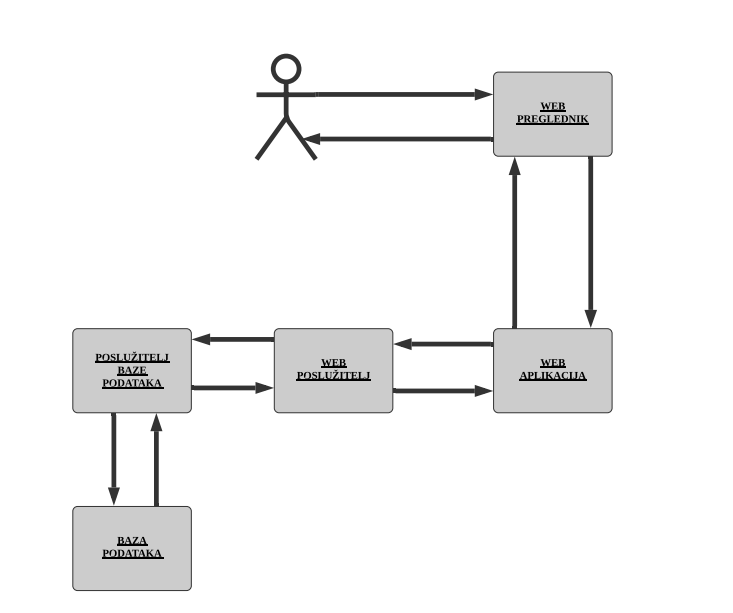
\includegraphics[scale=1.0]{slike/arh.PNG} %veličina slike u odnosu na originalnu datoteku i pozicija slike
			\centering
			\caption{Arhitektura sustava}
			\label{fig:promjene}
		\end{figure}
	Prilikom programiranja sustava prvo se bilo bitno dogovoriti oko korištene arhitekture i tehnologije koja će se za izradu web aplikacije koristiti. Odluke kao što su programski jezik i razvojno okruženje za korištenje same internet aplikacije. Arhitekturu smo odabrali kako bi zadovoljavala mnoge značajke kao što su fleksibilnost, mogućnost nadogradnje, što jeftinije održavanje. Web aplikacije nam se činila kao najlogičniji odabir iz razloga što ne ovisi o uređaju na kojem se prikazuje te se nismo morali opredijeljivati za operacijski sustav u kojem će raditi najefikasnije. Također odabrana arhitektura od korisnika naše web aplikacije zahtjeva samo pristup internet te internetski preglednik što je dostupno većini.  \newline
	\indent Pregled web-stranice te svih podataka i zatraženih medija odvija se uz pomoć \underbar{\textit{web preglednika}}. Web preglednik ima nekoliko uloga, jedna od njih je prikaz stranice na način čitljiv čovjeku. Stoga možemo reći da web preglednik ima funkciju prevoditelja. Također, upravo web preglednik je alat pomoću kojeg korisnik šalje zahtjev web poslužitelju. \newline
	\indent Iduća funkcionalnost je komunkacija s aplikacijom. Tome služi \underbar{\textit{web poslužitelj}} koji je poput motora web aplikacije. Sama komunikacija odvija se pomoću HTTP protokola koji služi za prijenos informacija i komunikaciju na internetu. \newline
	\indent \underbar{\textit{Web aplikacija}} se pokreće pomoću web poslužitelja koji joj prosljeđuje zahjtev, a sama web aplikacija služi za obradu zahtjeva prosljeđenih s web poslužitelja. Web aplikacija ima mogućnost pristupa bazi podataka. Podaci iz baze se kasnije prikazuju korisniku. Za sami prikaz je zaslužen već prije spomenuti web poslužitelj koji vraća korisniku HTML dokument kao odgovor, a čitljivi prikaz korisniku je osiguran pomoću web preglednika. \newline
	\indent Web aplikacija nam se sastoji od front-enda i back-enda. Tehnologija koju smo odabrali za izradu back-enda je Java Spring Boot, dok smo za front-end odabrali React.js. Arhitektura sustava za koju smo se odlučili je MVC odnosno (Model-View-Controller) koncept. \newline
	\indent Glavna korist MVC kocepta je ta što dijelovi aplikacije nisu usko povezani te se lakše testiraju, a i greška u jednom od dijelova neće utjecati na rad ostalih. \newline
	MVC koncept sastoji se od:
	\begin{itemize}
		\item   \textbf{Model} - klase koje opisuju same podatke koji se koriste u aplikaciji. Klase također sadrže i logiku vezanu za te podatke. Podaci u modelu ne ovise o korisničkom sučelju. Model prima ulazne podatke od Controllera.
		\item 	\textbf{View} - omogućuje komunikaciju s korisnikom te definira kako će korisničko sučelje biti prikazano korisniku.
		\item 	\textbf{Controller}	- klase koje kontroliraju komunikaciju korisnika sa aplikacijom. To je sloj aplikacije koji obrađuje korisničke zahtjeve. Controller prihvaća sve ulaze i pretvara ih u naredbe za Model i View.   	
	\end{itemize}

	
		\section{Baza podataka}
		Za potrebe WebGym sustava koristit ćemo relacijsku bazu podataka koja nam pojednostavljuje modeliranje odnosa i scenarija koji se u realnosti dešavaju. Svaka je tablica definirana svojim imenom te skupom atributa koji su nam potrebni za punu funkcionalnost pojma ili odnosa opisanim tablicom. Brza i jednostavna pohrana te pristup samim podacima je zadaća ovog sustava pohranjivanja podataka u bazu. Baza podataka sastoji se od sljedećih entiteta:
		\begin{itemize}
	        	\item 	Korisnik
	        	\item 	Teretana 
	        	\item 	TeretanaLokacija 
	        	\item   Ciljevi
	        	\item 	PlanTreningaIPrehrane
	        	\item 	Članarina
	        	\item 	ČlanarinaKlijent
	        	\item 	Zamolba
	        	\item   PlanKlijent
	        	\item   TeretanaKorisnik
        	\end{itemize}
		
		
		\subsection{Opis tablica}
		\textbf{Korisnik} Ovaj entitet sadržava sve bitne informacije o korisniku WebGym web aplikacije. Sadrži atribute kao što su: korisničko ime, ime, prezime, email, hashiranu lozinku, broj mobitela, broj PayPala, visinu, težinu te ulogu u sustavu. U ulozi ovise ovlasti koje korisnik u sustavu i u odnosima ima. Ovaj entitet je u vezi \emph{One-to-Many} s entitetom Ciljevi preko korisničkog imena klijenta koji je i sam korisnik, u vezi s \emph{Many-to-Many} entitetom PlanTreningaIPrehrane preko korisničkog imena trenera koji je i sam korisnik, u vezi \emph{One-to-Many} s entitetom ČlanarinaKlijent preko korisničkog imena klijenta, u vezi \emph{One-to-Many} s entitetom  Zamolba korisničkog imena trenera, u vezi \emph{Many-to-Many} s entitetom PlanKlijent preko korisničkog imena klijenta te u vezi \emph{Many-to-Many} s entitetom TeretanaKorisnik preko korisničkog imena trenera ili voditelja koji su i sami korisnici.
				
				
    			\begin{longtabu} to \textwidth {|X[10, l]|X[6, l]|X[20, l]|}
    					
    				\hline \multicolumn{3}{|c|}{\textbf{Korisnik}}	 \\[3pt] \hline
    				\endfirsthead
    					
    				\hline \multicolumn{3}{|c|}{\textbf{Korisnik}}	 \\[3pt] \hline
    				\endhead
    					
    				\hline 
    				\endlastfoot
    					
    					\cellcolor{LightGreen}korisničkoIme  & VARCHAR	&  	jedinstveno ime korisnika 	\\ \hline
    					ime	& VARCHAR & ime korisnika  	\\ \hline 
    					prezime & VARCHAR & prezime korisnika   \\ \hline 
    					email & VARCHAR	&  	email korisnika s kojim je napravio račun	\\ \hline 
    					lozinka	& VARCHAR & hash korisnikove lozinke za prijavu  	\\ \hline
    					brojMobitela	& VARCHAR & korisnikov broj mobitela  	\\ \hline
    					PayPal	& VARCHAR & korisnikov PayPal za plaćanje usluga  	\\ \hline
    					visina	& INT & korisnikova težina  	\\ \hline
    					težina	& INT & korisnikova visina  	\\ \hline
    					uloga	& VARCHAR & korisnikova uloga u sustavu  	\\ \hline
					
					
				\end{longtabu}
				
				\textbf{Teretana} ovaj entitet sadrži sve bitne informacije o lancu teretani. Sadrži atribute: id, ime, opis te email, a ovaj je entitet u vezi \emph{One-to-Many} s entitetom TeretanaLokacija preko jedinstvenog brojčanog identifikatora teretane te u vezi \emph{One-to-Many} s entitetom članarina preko jedinstvenog brojčanog identifikatora teretane.
				\begin{longtabu} to \textwidth {|X[10, l]|X[6, l]|X[20, l]|}
    					
    				\hline \multicolumn{3}{|c|}{\textbf{Teretana}}	 \\[3pt] \hline
    				\endfirsthead
    					
    				\hline \multicolumn{3}{|c|}{\textbf{Teretana}}	 \\[3pt] \hline
    				\endhead
    					
    				\hline 
    				\endlastfoot
    					
    					\cellcolor{LightGreen}id  & INT	&  	jedinstveni brojčani identifikator teretane 	\\ \hline
    					ime	& VARCHAR & ime teretane  	\\ \hline 
    					opis & VARCHAR & opis teretane   \\ \hline 
    					email & VARCHAR	&  	e mail teretane	\\ \hline 
					
					
				\end{longtabu}
				
			\textbf{TeretanaLokacija} ovaj entitet sadrži sve bitne informacije o pojedinoj teretani. Sadrži atribute: id,id lanca teretani, država u kojoj se nalazi, grad u kojem se nalazi, ulica u kojoj se nalazi, početak ranog vremena teretane, kraj radnog vremena teretane te broj telefona teretane, a ovaj je entitet u vezi \emph{Many-to-One} s entitetom Teretana preko jedinstvenog brojčanog identifikatora teretane, u vezi \emph{One-to-Many} s entitetom Zamolba preko jedinstvenog brojčanog identifikatora pojedine teretane te je u vezi \emph{One-to-Many} s entitetom TeretanaKorisnik preko jedinstvenog brojčanog identifikatora pojedine teretane.
			\begin{longtabu} to \textwidth {|X[10, l]|X[6, l]|X[20, l]|}
    					
    				\hline \multicolumn{3}{|c|}{\textbf{TeretanaLokacija}}	 \\[3pt] \hline
    				\endfirsthead
    					
    				\hline \multicolumn{3}{|c|}{\textbf{TeretanaLokacija}}	 \\[3pt] \hline
    				\endhead
    					
    				\hline 
    				\endlastfoot
    					
    					\cellcolor{LightGreen}id  & INT	&  	jedinstveni brojčani identifikator pojedine teretane 	\\ \hline
    					\cellcolor{LightBlue} idTeretana	& INT & jedinstveni brojčani identifikator lanca teretani (Teretana.id)  	\\ \hline 
    					država & VARCHAR & država u kojoj se teretana nalazi   \\ \hline 
    					grad & VARCHAR	&  	grad u kojem se teretana nalazi	\\ \hline 
    					ulica	& VARCHAR & ulica u kojoj se teretana nalazi  	\\ \hline
    					radnoVrijemePočetak	& TIME & vrijeme početka rada teretane  	\\ \hline
    					radnoVrijemeKraj	& TIME & vrijeme kraja rada teretane  	\\ \hline
    					telefon	& VARCHAR & broj na koji se teretana može nazvati  	\\ \hline
					
					
			\end{longtabu}
			
			\textbf{Ciljevi} ovaj entitet sadrži sve važne informacije o ciljevima samog klijenta. Sadrži atribute: id,korisničko ime klijenta te opis cilja, a ovaj je entitet u vezi \emph{Many-to-One} s entitetom Korisnik preko korisničkog imena.
			\begin{longtabu} to \textwidth {|X[10, l]|X[6, l]|X[20, l]|}
    					
    				\hline \multicolumn{3}{|c|}{\textbf{Ciljevi}}	 \\[3pt] \hline
    				\endfirsthead
    					
    				\hline \multicolumn{3}{|c|}{\textbf{Ciljevi}}	 \\[3pt] \hline
    				\endhead
    					
    				\hline 
    				\endlastfoot
    					
    					\cellcolor{LightGreen}id  & INT	&  	jedinstveni brojčani identifikator cilja 	\\ \hline
    					\cellcolor{LightBlue} korisničkoImeKlijent	& VARCHAR & jedinstveni brojčani identifikator klijenta koji cilj obavlja (Korisnik.korisničkoIme)  	\\ \hline 
    					opis & VARCHAR & opis cilja   \\ \hline 
    					obavljeno & BOOLEAN	& je li cilj obavljen	\\ \hline 
					
					
			\end{longtabu}
			
			
			\textbf{PlanTreningaIPrehrane} ovaj entitet sadrži sve važne informacije o planu treninga i prehrane. Korisnik može kupiti trening te onda ima individualni pristup trenera, ili može samo kupiti plan te dobiti gotov file sa treninzima i preporučenim načinom prehrane. Sadrži atribute: id,korisničko ime trenera, opis plana, datum početka plana, datum isteka plana te atribut koji nam govori je li trening u pitanju, a ovaj je entitet u vezi \emph{Many-to-Many} s entitetom Korisnik preko korisničkog imena.
			\begin{longtabu} to \textwidth {|X[10, l]|X[6, l]|X[20, l]|}
    					
    				\hline \multicolumn{3}{|c|}{\textbf{PlanTreningaIPrehrane}}	 \\[3pt] \hline
    				\endfirsthead
    					
    				\hline \multicolumn{3}{|c|}{\textbf{PlanTreningaIPrehrane}}	 \\[3pt] \hline
    				\endhead
    					
    				\hline 
    				\endlastfoot
    					
    					\cellcolor{LightGreen}id  & INT	&  	jedinstveni brojčani identifikator plana treninga i prehrane 	\\ \hline
    					\cellcolor{LightBlue} korisničkoImeTrener 	& VARCHAR & jedinstveni brojčani identifikator trenera čiji je plan (Korisnik.korisničkoIme)  	\\ \hline 
    					opis & VARCHAR & opis plana treninga i prehrane   \\ \hline 
    					datumPočetka & TIMESTAMP & vrijeme početka plana   \\ \hline
    					datumIsteka & TIMESTAMP & vrijeme kraja plana   \\ \hline
    					cijena & DECIMAL & cijena plana   \\ \hline
    					jeLiTrening & BOOLEAN	& je li plan individalni plan, inače je samo kupljeni gotovi plan treninga i prehrane	\\ \hline
					
					
			\end{longtabu}
			
			\textbf{Članarina} ovaj entitet sadrži sve važne informacije o članarini u teretani.  Sadrži atribute: id,id pojedine teretane, cijena članarine, opis te trajanje, a ovaj je entitet u vezi \emph{Many-to-One} s entitetom Teretana preko jedinstvenog brojčanog identifikatora teretane te je u vezi \emph{One-to-Many} s entitetom ČlanarinaKlijent preko jedinstvenog brojčanog identifikatora članarine.
			\begin{longtabu} to \textwidth {|X[10, l]|X[6, l]|X[20, l]|}
    					
    				\hline \multicolumn{3}{|c|}{\textbf{Članarina}}	 \\[3pt] \hline
    				\endfirsthead
    					
    				\hline \multicolumn{3}{|c|}{\textbf{Članarina}}	 \\[3pt] \hline
    				\endhead
    					
    				\hline 
    				\endlastfoot
    					
    					\cellcolor{LightGreen}id  & INT	&  	jedinstveni brojčani identifikator članarine 	\\ \hline
    					\cellcolor{LightBlue} idTeretana  	& INT & jedinstveni brojčani identifikator trenere koja nudi članarinu (Teretana.id)  	\\ \hline
    					cijena & DECIMAL & cijena članarine   \\ \hline
    					opis & VARCHAR & opis članarine (što se članarina uključuje)   \\ \hline
    					trajanje & INTERVAL & trajanje članarine   \\ \hline
					
					
			\end{longtabu}
			
			\textbf{ČlanarinaKlijent} ovaj entitet sadrži sve važne informacije o članarini koju klijent posjeduje. Sadrži atribute: id,korisničko ime klijenta, id članarine koju teretana nudi, datum početka te dazum isteka trajanja članarine, a ovaj je entitet u vezi \emph{Many-to-One} s entitetom Korisnik preko korisničkog imena klijenta te je u vezi \emph{Many-to-One} s entitetom Članarina preko jedinstvenog brojčanog identifikatora članarine.
			\begin{longtabu} to \textwidth {|X[10, l]|X[6, l]|X[20, l]|}
    					
    				\hline \multicolumn{3}{|c|}{\textbf{ČlanarinaKlijent}}	 \\[3pt] \hline
    				\endfirsthead
    					
    				\hline \multicolumn{3}{|c|}{\textbf{ČlanarinaKlijent}}	 \\[3pt] \hline
    				\endhead
    					
    				\hline 
    				\endlastfoot
    					
    					\cellcolor{LightGreen}id  & INT	&  	jedinstveni brojčani identifikator članarine koju klijent posjeduje 	\\ \hline
    					\cellcolor{LightBlue} korisničkoImeKlijent  	& VARCHAR & korisničko ime klijenta koji posjeduje članarinu (Korisnik.korisničkoIme)  	\\ \hline
    					\cellcolor{LightBlue} idČlanarina  	& INT & jedinstveni brojčani identifikator članarine (Članarina.id)    \\ \hline
					    datumPočetka & TIMESTAMP & datum početka trajanja članarine   \\ \hline
    					datumIsteka & TIMESTAMP & datum kraja trajanja članarine   \\ \hline
					
			\end{longtabu}
			
			\textbf{Zamolba} ovaj entitet sadrži sve važne informacije o prijavi za posao koju trener šalje pojedinoj teretani. Sadrži atribute: id,korisničko ime trenera, id pojedine teretane u kojoj se trener za posao prijavljuje, te opis prijave, a ovaj je entitet u vezi \emph{Many-to-One} s entitetom Korisnik preko korisničkog imena trenera te je u vezi \emph{Many-to-One} s entitetom Teretana preko jedinstvenog brojčanog identifikatora teretane.
			\begin{longtabu} to \textwidth {|X[10, l]|X[6, l]|X[20, l]|}
    					
    				\hline \multicolumn{3}{|c|}{\textbf{Zamolba}}	 \\[3pt] \hline
    				\endfirsthead
    					
    				\hline \multicolumn{3}{|c|}{\textbf{Zamolba}}	 \\[3pt] \hline
    				\endhead
    					
    				\hline 
    				\endlastfoot
    					
    					\cellcolor{LightGreen}id  & INT	&  	jedinstveni brojčani identifikator prijave 	\\ \hline
    					\cellcolor{LightBlue} korisničkoImeTrener 	& VARCHAR & korisničko ime trenera koji se prijavljuje za posao u teretani (Korisnik.korisničkoIme)  	\\ \hline
    					\cellcolor{LightBlue} idTeretana  	& INT & jedinstveni identifikator teretane u koju se prijavljuje (TeretanaLokacija.id)    \\ \hline
					    opis & VARCHAR & opis prijave za posao   \\ \hline
    					dozvola & BOOLEAN & je li treneru odobren rad u teretani   \\ \hline
					
			\end{longtabu}
			
			\textbf{PlanKlijent} ovaj entitet sadrži sve važne informacije o planu prehrane i treninga kojeg klijent posjeduje. Sadrži atribute: id, id plana, korisničko ime klijenta, te datum kupnje, a ovaj je entitet u vezi \emph{Many-to-One} s entitetom Korisnik preko korisničkog imena klijenta te je u vezi  \emph{Many-to-One} s entitetom PlanTreningaIPrehrane preko jedinstvenog brojčanog identifikatora plana.
			\begin{longtabu} to \textwidth {|X[10, l]|X[6, l]|X[20, l]|}
    					
    				\hline \multicolumn{3}{|c|}{\textbf{PlanKlijent}}	 \\[3pt] \hline
    				\endfirsthead
    					
    				\hline \multicolumn{3}{|c|}{\textbf{PlanKlijent}}	 \\[3pt] \hline
    				\endhead
    					
    				\hline 
    				\endlastfoot
    					
    					\cellcolor{LightGreen}id  & INT	&  	jedinstveni brojčani identifikator plana kojeg klijent posjeduje 	\\ \hline
    					\cellcolor{LightBlue} idPlan 	& INT & jedinstveni brojčani identifikator plana treninga i prehrane (PlanTreningaIPrehrane.id)  	\\ \hline
    					\cellcolor{LightBlue} korisničkoImeKlijent  & VARCHAR & korisničko ime klijenta koji plan posjeduje (Korisnik.korisničkoIme) \\ \hline
					    datumKupnje & TIMESTAMP & datum kupnje plana   \\ \hline
		    \end{longtabu}
			
			\textbf{TeretanaKorisnik} ovaj entitet sadrži sve važne informacije o korisniku koji radi u teretani kao voditelj ili kao trener. Sadrži atribute: id, id pojedine teretane, korisničko ime korisnika, te datum početka rada, a ovaj je entitet u vezi \emph{Many-to-One} s entitetom Korisnik preko korisničkog imena korisnika te je u vezi \emph{Many-to-One} s entitetom TeretanaLokacija preko jedinstvenog brojčanog identifikatora pojedine teretane.
			\begin{longtabu} to \textwidth {|X[10, l]|X[6, l]|X[20, l]|}
    					
    				\hline \multicolumn{3}{|c|}{\textbf{TeretanaKorisnik}}	 \\[3pt] \hline
    				\endfirsthead
    					
    				\hline \multicolumn{3}{|c|}{\textbf{TeretanaKorisnik}}	 \\[3pt] \hline
    				\endhead
    					
    				\hline 
    				\endlastfoot
    					
    					\cellcolor{LightGreen}id  & INT	&  	jedinstveni brojčani identifikator odnosa korisnika i teretane 	\\ \hline
    					\cellcolor{LightBlue} idTeretana 	& INT & jedinstveni brojčani identifikator plana treninga i prehrane (TeretanaLokacija.id)  	\\ \hline
    					\cellcolor{LightBlue} korisničkoImeKorisnik  & VARCHAR & korisničko ime trenera ili voditelja u teretani (Korisnik.korisničkoIme)   \\ \hline
					    datumPočetkaRada & TIMESTAMP & datum zaposlenja trenera u teretani   \\ \hline
					
			\end{longtabu}
			
			
			\subsection{Dijagram baze podataka}
				\textit{ U ovom potpoglavlju potrebno je umetnuti dijagram baze podataka. Primarni i strani ključevi moraju biti označeni, a tablice povezane. Bazu podataka je potrebno normalizirati. Podsjetite se kolegija "Baze podataka".}
			
			\eject
			
			
		\section{Dijagram razreda}
		
			\textit{Potrebno je priložiti dijagram razreda s pripadajućim opisom. Zbog preglednosti je moguće dijagram razlomiti na više njih, ali moraju biti grupirani prema sličnim razinama apstrakcije i srodnim funkcionalnostima.}\\
			
			\textbf{\textit{dio 1. revizije}}\\
			
			\textit{Prilikom prve predaje projekta, potrebno je priložiti potpuno razrađen dijagram razreda vezan uz \textbf{generičku funkcionalnost} sustava. Ostale funkcionalnosti trebaju biti idejno razrađene u dijagramu sa sljedećim komponentama: nazivi razreda, nazivi metoda i vrste pristupa metodama (npr. javni, zaštićeni), nazivi atributa razreda, veze i odnosi između razreda.}\\
			
			\textbf{\textit{dio 2. revizije}}\\			
			
			\textit{Prilikom druge predaje projekta dijagram razreda i opisi moraju odgovarati stvarnom stanju implementacije}
			
			
			
			\eject
		
		\section{Dijagram stanja}
			
			
			\textbf{\textit{dio 2. revizije}}\\
			
			\textit{Potrebno je priložiti dijagram stanja i opisati ga. Dovoljan je jedan dijagram stanja koji prikazuje \textbf{značajan dio funkcionalnosti} sustava. Na primjer, stanja korisničkog sučelja i tijek korištenja neke ključne funkcionalnosti jesu značajan dio sustava, a registracija i prijava nisu. }
			
			
			\eject 
		
		\section{Dijagram aktivnosti}
			
			\textbf{\textit{dio 2. revizije}}\\
			
			 \textit{Potrebno je priložiti dijagram aktivnosti s pripadajućim opisom. Dijagram aktivnosti treba prikazivati značajan dio sustava.}
			
			\eject
		\section{Dijagram komponenti}
		
			\textbf{\textit{dio 2. revizije}}\\
		
			 \textit{Potrebno je priložiti dijagram komponenti s pripadajućim opisom. Dijagram komponenti treba prikazivati strukturu cijele aplikacije.}